
\documentclass[10pt]{beamer}

\usetheme[progressbar=frametitle]{metropolis}
\usepackage{appendixnumberbeamer}

\usepackage{booktabs}
\usepackage[scale=2]{ccicons}
\usepackage{relsize}
\usepackage{pgfplots}
\usepgfplotslibrary{dateplot}



\usepackage{multicol}
\usepackage{lmodern}
\usepackage{lipsum}
\usepackage{marvosym}
\usepackage{adjustbox}
\usepackage{nicefrac}
\usepackage{upgreek}


\usepackage{xspace}
\newcommand{\themename}{\textbf{\textsc{metropolis}}\xspace}

\usepackage[T1]{fontenc}
\usepackage[sfdefault,condensed]{roboto}

%\usepackage{FiraSans}
\usepackage{pgf} 
\usepackage{amsmath}
\usepackage{adjustbox}

\title %optional
{\textsc{Unravelling the contribution of \\financial and longevity risks\\ to changes over time \\in life annuities}}
 
%\subtitle{A short story}
 
\author % (optional, for multiple authors)
{Jes\'us-Adri\'an \'Alvarez \\ \and Andr\'es M. Villegas\\ \href{mailto:alvarez@sdu.dk}{alvarez@sdu.dk}}
 

 
 
\date{} % (optional)

 
%\logo{\includegraphics[height=1.5cm]{SDU-logo.png}}
%\titlegraphic{\hfill\includegraphics[height=1.5cm]{SDUDKUKunder.pdf}}

 
 
 
%\logo{\pgfputat{\pgfxy(9.45,1.5)}{\pgfbox[center,base]{\includegraphics[width=1.7cm]{SDUDKUKunder.pdf}}}}

\begin{document}


\maketitle

%\section{Introduction}

\metroset{titleformat frame=allsmallcaps}


{\setbeamercolor{palette primary}{fg=white, bg=black}
	\begin{frame}[standout]
\scalebox{3}{stochastic}
\scalebox{3}{change}
\scalebox{3}{life annuities}
%\scalebox{2}{interest           mortality}
\end{frame}
}


{\setbeamercolor{palette primary}{fg=white, bg=black}
	\begin{frame}[standout]
	\scalebox{2.5}{interest or  mortality?}
\end{frame}
}


\begin{frame}{Life annuity factors}

\begin{center}\nonumber
	\scalebox{2}{$\bar{a}_x(t) = \int_0^\infty {}_sp_x(t) {v}(s,t)ds$} \nonumber
\end{center} 


\scalebox{2}{$\underbrace{e^{-\int_{0}^{s}\delta(y,t)dy}}_\text{interest}$}


\scalebox{2}{$\underbrace{e^{-\int_{0}^{s}\mu(x+y,t)dy}}_\text{mortality}$}





\end{frame}



\section{Duration}

\begin{frame}{Duration: Sensitivity of $\bar{a}_x(t)$ to constant changes in $\delta$}


\begin{center}\nonumber
\scalebox{1.5}{${D}_{x}(t) = -\frac{ \frac{\partial \bar{a}_x(t) }{\partial \delta}}{\bar{a}_x(t)}$}
\end{center} \pause





\begin{center}
\textit{The \textbf{greater} ${D}_{x}(t)$, the \textbf{more sensitive} $\bar{a}_x(t)$ is to changes in $\delta$}.\pause
\end{center}




Interest rate immunization {\scriptsize (Redington, 1951; Fisher, 1971; Shiu et al. 1991; Courtouis 2007)}: \pause

\begin{itemize}
	\item \textbf{Modified Duration:} ${D}_{x}(t) = -\frac{\int_0^\infty s {}_sp_x(t) {v}(s,t)ds}{\bar{a}_x(t)}$\pause
	

	\item \textbf{Dollar Duration}: ${D}_{x}(t)\bar{a}_x(t)$.\pause
\end{itemize}


How annuities respond to\textbf{ changes in interest rates}? {\scriptsize(Milevsky, 2013; Charupat, Kamstra, Milevsky, 2015)}


\end{frame}

\section{What about changes in mortality?}

\section{Results from Demography}


\begin{frame}{Lifetable entropy}
	
	\textbf{Life expectancy}
	\begin{center}\nonumber
		\scalebox{1.5}{$e_0 = \int_0^\infty {}_sp_xds$} \pause
	\end{center} 


	\textbf{Lifetable entropy}
	
	\begin{center}\label{eq:EntropyGeneral}
	\scalebox{1.5}{${H} = \frac{ \frac{\partial e_0 }{\partial \mu}}{e_0} = \dfrac{\int_0^\infty e(x) f(x)ds}{e_0}$}. \pause
	\end{center}
	
	\begin{center}
	"Sensitivity of \textbf{life expectancy} to proportional changes in the \textbf{force of mortality} {\scriptsize (Keyfitz, 1977; Demetrius, 1976)}" \pause
	\end{center}

	
	
	
\textbf{Variation in individual lifespans} {\scriptsize (Vaupel, 1986)}: \pause
\begin{itemize}
	\item \textbf{Inverse relationship}: $e_0$ increase $\rightarrow$ $H$ decline, {\scriptsize (Colchero et al, 2016; Aburto et al, 2020)} \pause
	\item Comparison of \textbf{ageing patterns across species.} {\scriptsize (Baudisch et al, 2011)}
\end{itemize}
	
\end{frame}


\begin{frame}{Changes over time in $e_0(t)$}

\textbf{Changes over time}

\begin{center}
	\scalebox{1.5}{$\dot{e}_0(t) = \frac{\partial e_0(t)}{\partial t}$}\pause
\end{center}


Vaupel and Canudas-Romo (2003) showed that:

\begin{center}
	\scalebox{1.5}{$\dot{e}_0(t) =\bar{\rho}(t) H(t) + Cov(\rho, e_0(t))$}, \pause
\end{center}


where 

\begin{itemize}
	\item $\bar{\rho}(t)$, \textbf{average mortality improvement at all ages}, \pause
	\begin{itemize}
		\item $\rho(x,t)= \frac{-\dfrac{\partial \mu(x,t)}{\partial t}}{\mu(x,t)}$, \textbf{rate mortality improvement at age x}, \pause
	\end{itemize}
	
	\item $H$: \textbf{entropy}. \pause
\end{itemize}

\textbf{Extended to causes-of-death and subpopulations (e.g. socio-economic groups)}.
\end{frame}



\section{Entropy of life annuity}

\begin{frame}{Entropy of life annuity}

Haberman et al (2011) extended the concept \textbf{of entropy to life annuities}: \pause

\begin{center}
\scalebox{1.5}{${H}_{x}(t) = \frac{ \frac{\partial \bar{a}_x(t) }{\partial \delta}}{\bar{a}_x(t)}$}
\end{center}

\begin{center}
\textit{"Sensitivity of $\bar{a}_x(t)$ to proportional changes in $\delta$"}\pause
\end{center}

They showed that


\begin{center}
	\scalebox{1.5}{${H}_{x}(t) =  \frac{\int_0^\infty \mu(x+s,t)  {}_sp_x(t) {v}(s,t)  \bar{a}_x(t) ds}{\bar{a}_x(t)}$}, \pause
\end{center}

\end{frame}


\section{Longevity immunization}

\begin{frame}{Longevity immunization}
Increasing awareness of \textbf{longevity risk} {\scriptsize(Blake, Cairns,Down and Kessler, 2019)}:\pause

\begin{itemize}
	\item low interest rates, \pause
	\item continuous mortality improvements, \pause
	\item increased exposure to \textbf{unexpected changes in mortality}. \pause
\end{itemize}


Key Q-duration {\scriptsize(Li and Luo, 2011)} \pause

Longevity Greeks {\scriptsize(Zhou and Li, 2019)} \pause



\textbf{Longevity immunization:} Strategies to ensure that the value of portfolio will be little affected in response to changes in mortality {\scriptsize (Wang, 2010; Tsai et al 2011; Li et al, 2011)}\pause
	
	\begin{itemize}
		\item \textbf{Mortality Duration = Entropy} {\scriptsize(Haberman, 2011)} \pause
		\item \textbf{No reference to any demographic study! } \pause
		\item \textbf{Only focused on changes in mortality}, \pause
		\item Lin and Tsai (2020) sensitivity to changes in the \\ \textit{force of mortality-interest}: $\mu^{*}=\mu+\delta$.
	\end{itemize}
	
\end{frame}


\section{Decomposition of changes \\ over time in $\bar{a}_x(t)$}


\begin{frame}{Changes over time in $\bar{a}_x(t)$}

\textbf{Derivative of $\bar{a}_x(t)$ with respect to time $t$:}

\begin{center}
	\scalebox{2}{$\dot{\bar{a}}_x(t) = \frac{\partial \bar{a}_x(t)}{\partial t}$}\pause
\end{center}

\textbf{Relative derivative of $\bar{a}_x(t)$:}

\begin{center}
	\scalebox{2}{$\acute{\bar{a}}_x(t) = \frac{\dot{\bar{a}}_x(t)}{\bar{a}_x(t)}$}
\end{center}

\end{frame}


{\setbeamercolor{palette primary}{fg=white, bg=black}
	\begin{frame}[standout]
	\scalebox{2.5}{putting all the}
		\scalebox{2.5}{pieces together...}
\end{frame}
}



\begin{frame}{Decomposition of changes over time in $\bar{a}_x(t)$}

\begin{center}
	\scalebox{2}{$\acute{\bar{a}}_x(t) = \underbrace{\bar{\upvarphi}(t){D}_x(t)}_\text{financial component}+\underbrace{\bar{\rho}(t){H}_x(t)}_\text{longevity component}
		$}\pause
\end{center}

where

\begin{itemize}

	\item $\bar{\upvarphi}(t)$\textbf{: relative change in the term-structure of interest rates,} \pause
	\item ${D}_x(t)$\textbf{: duration of $\bar{a}_x(t)$,}	\pause
	\item $\bar{\rho}(t)$\textbf{: average mortality improvement at all ages above $x$,} \pause
	\item ${H}_x(t)$\textbf{: entropy of $\bar{a}_x(t)$.} \pause
\end{itemize}


\textbf{Stochastic changes} in $\bar{a}_x(t)$ are driven by $\bar{\upvarphi}(t)$ and $\bar{\rho}(t)$, which are \textbf{modulated} by  ${D}_x(t)$ and ${H}_x(t)$.
\end{frame}






\begin{frame}{Decomposition of changes over time in $\bar{a}_x(t)$}


If $v(s,t)=e^{-\delta(t)s}$, then 


\begin{center}
	\scalebox{2}{$\acute{\bar{a}}_x(t) = \underbrace{\dot{\delta}(t){D}_x(t)}_\text{financial component}+\underbrace{\bar{\rho}(t){H}_x(t)}_\text{longevity component}
		$}\pause
\end{center}

where

\begin{itemize}
	
	\item $\dot{\delta}(t)=\dfrac{\partial \delta(t)}{\partial t}$\textbf{: change over time in interest rates $x$,} \pause
	\item ${D}_x(t)$\textbf{: Modified duration of $\bar{a}_x(t)$,}	\pause
	\item $\bar{\rho}(t)$\textbf{: average mortality improvement at all ages above $x$,} 
	\item ${H}_x(t)$\textbf{: entropy of $\bar{a}_x(t)$} \pause
\end{itemize}

It suffices to use the \textbf{modified duration} ($D_x(t)$) and \textbf{entropy} (${H}_x(t)$) together with $\dot{\delta}(t)$ and $\bar{\rho}(t)$ to determine the contribution of \textbf{financial and longevity risks} to changes over time in \textbf{life annuities}. \pause

\textbf{No assumptions about the functional form of $\delta$ and $\mu$ (entirely data-driven).}
\end{frame}







\section{Historical contributions to changes in life annuities in the UK}


\begin{frame}{Historical contributions of mortality and interest rates}
\textbf{Data}
\begin{itemize}
	\item \textbf{Long-term interest rates:} the yield on 2.5\% Consols up to 1977, then by the yield on FTSE Actuaries Government Securities Irredeemable stocks up to 2014 and thereafter by the yield on FTSE Actuaries Government Securities 45 years stock (Bank of England, 2020), \pause
	\item \textbf{Mortality rates: } Human Mortality Database (2020), \pause
	\item \textbf{1841-2018.}
\end{itemize}


\end{frame}


\begin{frame}{Interest and mortality rates for females in the UK, 1841-2018}
\begin{figure}
	\centering
	\hspace*{-0.8cm}
	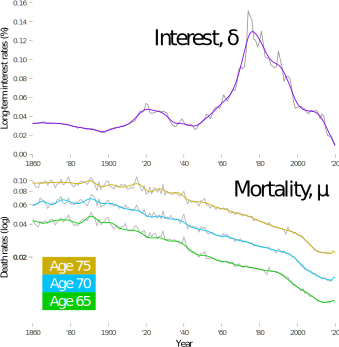
\includegraphics[scale=0.9] {Fig0.pdf}
\end{figure}
\end{frame}


\begin{frame}{Interest and mortality rates for males in the UK, 1841-2018}
\begin{figure}
	\centering
	\hspace*{-0.8cm}
	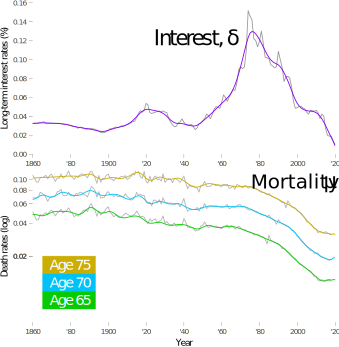
\includegraphics[scale=0.9] {Fig0m.pdf}
\end{figure}
\end{frame}



\begin{frame}{Life annuity factors at ages 65, 70 and 75. UK, 1841-2018}
\begin{figure}
	\centering
	\hspace*{-0.8cm}
	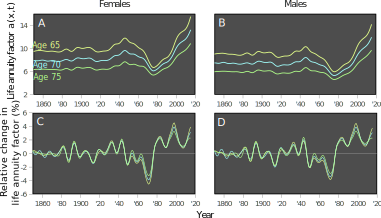
\includegraphics[scale=1.2] {Fig1.pdf}
\end{figure}
\end{frame}



\begin{frame}{Changes over time in interest and mortality rates. UK 1841-2018}
\begin{figure}
	\centering
	\hspace*{-0.8cm}
	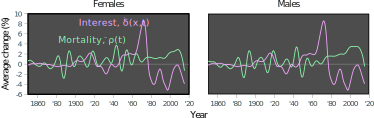
\includegraphics[scale=1.2] {Fig2.pdf}
\end{figure}
\end{frame}


\begin{frame}{Duration and Entropy at ages 65, 70 and 75. UK, 1841-2018}
\begin{figure}
	\centering
	\hspace*{-0.8cm}
	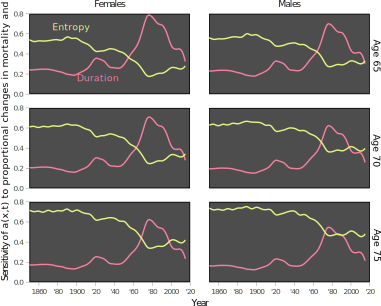
\includegraphics[scale=1] {Fig3.pdf}
\end{figure}
\end{frame}

\begin{frame}{Decomposition of $\acute{\bar{a}}_x(t)$ at ages 65, 70 and 75. UK, 1841-2018}
\begin{figure}
	\centering
	\hspace*{-0.8cm}
	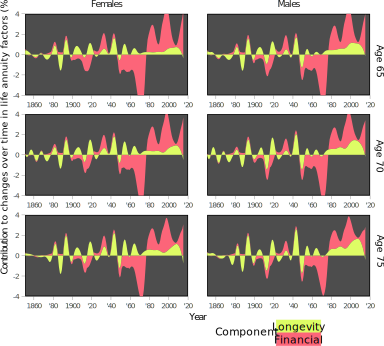
\includegraphics[scale=0.9] {Fig4.pdf}
\end{figure}
\end{frame}

\section{To sum up}

\begin{frame}{To sum up}

\textbf{Bringing results from demographic research to strengthen risk assessment} \pause
\begin{center}
	\scalebox{2}{$\acute{\bar{a}}_x(t) = \underbrace{\dot{\delta}(t){D}_x(t)}_\text{financial component}+\underbrace{\bar{\rho}(t){H}_x(t)}_\text{longevity component}
		$}\pause
\end{center}
\textbf{Stochastic changes} in $\bar{a}_x(t)$ are driven by $\dot{\delta}(t)$ and $\bar{\rho}(t)$, which are \textbf{modulated} by  ${D}_x(t)$ and ${H}_x(t)$. \pause


Thorough risk assessment: \textbf{financial and demographic sources of change}\\ $\rightarrow$ better \textbf{hedging strategies.} \pause

\textbf{No assumptions about the functional form of $\delta$ and $\mu$ (entirely data-driven).}



\end{frame}




\begin{frame}{To sum up}
\textbf{Historical developments}
\begin{itemize}
	\item \textbf{Longevity risk} has, most of the time, contributed to \textbf{increase} in $\bar{a}_x(t)$, but during some periods it has been \textbf{masked by high financial risk}. \pause
	\item Since the 1980s, \textbf{longevity risk contribute}s o most of the increases in $\bar{a}_x(t)$. \pause
	\begin{itemize}
		\item Increase in the number of papers/studies aiming at the quantification of longevity risk {\scriptsize (Blake, Cairns, Hunt, Kessel, 2019)} \pause
	\end{itemize}
	\item \textbf{At higher ages} (i.e. age 75 or older ages): \pause
	\begin{itemize}
		\item The sensitivity of $\bar{a}_x(t)$ to $\mu$ is higher, \pause
		\item Policies aiming at \textbf{increasing retirement ages entail higher longevity risk} (e.g. Denmark, Alvarez et al (2020)).
\end{itemize}
\end{itemize}
\end{frame}


\begin{frame}{Next steps}

\textbf{What about the future?}

\begin{itemize}
	\item Forecasting financial and longevity contributions under different models \pause
	\begin{itemize}
		\item Interest rates: Cox-Ingersol-Ross (CIR), \pause
		\item Mortality rates: CMI, APC, Lee-Carter and others with varying mortality improvements. \pause
	\end{itemize} 
\end{itemize}


\textbf{Extensions} \pause
\begin{itemize}
	\item Longevity contributions by \textbf{sub-population} (Sex-specific, by socio-economic groups), \pause
	\item \textbf{Causes of death} {\scriptsize Vaupel and Canudas-Romo (2003)}.
\end{itemize}


\end{frame}



\end{document}